%%
% 引言或背景
% 引言是论文正文的开端,应包括毕业论文选题的背景、目的和意义;对国内外研究现状和相关领域中已有的研究成果的简要评述;介绍本项研究工作研究设想、研究方法或实验设计、理论依据或实验基础;涉及范围和预期结果等。要求言简意赅,注意不要与摘要雷同或成为摘要的注解。
% modifier: 黄俊杰(huangjj27, 349373001dc@gmail.com)
% update date: 2017-04-15
%%

\chapter{绪论}
%定义,过去的研究和现在的研究,意义,与图像分割的不同,going deeper
\label{cha:introduction}
\section{课题背景}
\label{sec:background}
% What is the problem
% why is it interesting and important
% Why is it hards, why do naive approaches fails
% why hasn't it been solved before
% what are the key components of my approach and results, also include any specific limitations,do not repeat the abstract
%contribution
\subsection{光声成像简介}
光声成像的物理基础是光声效应。光声效应是最早由A.G.Bell于19世纪20年代所发现的物理现象。所谓光声效应,即当物体接受激光脉冲等光源照射后,因吸收光源的能量发生热弹性膨胀,产生压力波并通过物体传播的现象。如果利用激光束照射生物体,使其产生光声效应后,使用完全或部分围绕生物体表面S(常被称为采集表面)上的声学传感器记录随时间t所发生的压力变化$p(x,t)$。并根据声学测量数据$p(x,t)$重建初始压力$f(x)$,从而得到生物体成像的方法,就称为光声成像。

虽然光声效应被发现已久,但光声成像技术在近年来才得以被重视,并由于其高分辨率、高对比度的成像与无损害、无辐射的优势开始迅速发展。虽然如今的光声成像技术大多局限于研究领域,但随着光声成像技术的成熟,光声成像技术必将拥有更广阔的前景,在未来必将广泛地应用于临床医学检测领域。

\subsection{光声成像的优势}
现今我们已经掌握了多项成熟且完善的医学成像方法,包括广泛运用于医疗场所的利用X射线的CT成像技术,超声波扫描技术,核磁共振成像技术等,还有不太为公众所知的PET等技术。抛开现有的成熟技术,转而开发新的光声层析成像方法(PAT)是否是必要的呢?一个主要的答案是光声层析成像具有其他成像方法所不具备的优点。

\subsubsection{光声层析成像作为一种“混合”成像方法,能有效避免单一成像方法的弊端}
现有的成像方法大都依赖于某一种物理方法,而单一的物理方法所能得到的测量信息是有局限的。例如,由于许多肿瘤细胞比健康细胞在某些特定的能带上能吸收更多的电磁能量,因此使用电磁波的成像方法可以提供非常高的对比度,但由于电磁波的特性,这类成像方法只能提供非常低的分辨率。

如何规避单种物理方法所带来的局限性呢?一个显而易见的改进方法是同时使用多种物理过程成像,这种成像模式被称为“混合”成像方法(Hybrid imaging methods),而光声层析成像正是一种新兴的“混合”成像方法。光声层析成像同时使用了光波与声波两种物理波,即使用电磁波照射病灶,而后基于声学测量重建图像。事实上,由于癌细胞对激光能量的高吸收率,因此光声成像能产生高对比度的图像(此时单独使用超声波无法产生良好的对比度),并且通过超声波测量还获得了良好的分辨率(而激光波对于高分辨率图像来说太长了)。因此光声成像通过使用两种类型的波,在结合了它们优点的同时,消除了它们各自的缺点。如图\ref{img101},光声成像的两种实现模态(PACT、PAM)与其他的成像模态相比,具有更高的深度分辨率比。

\begin{figure}[h]
	\centering
	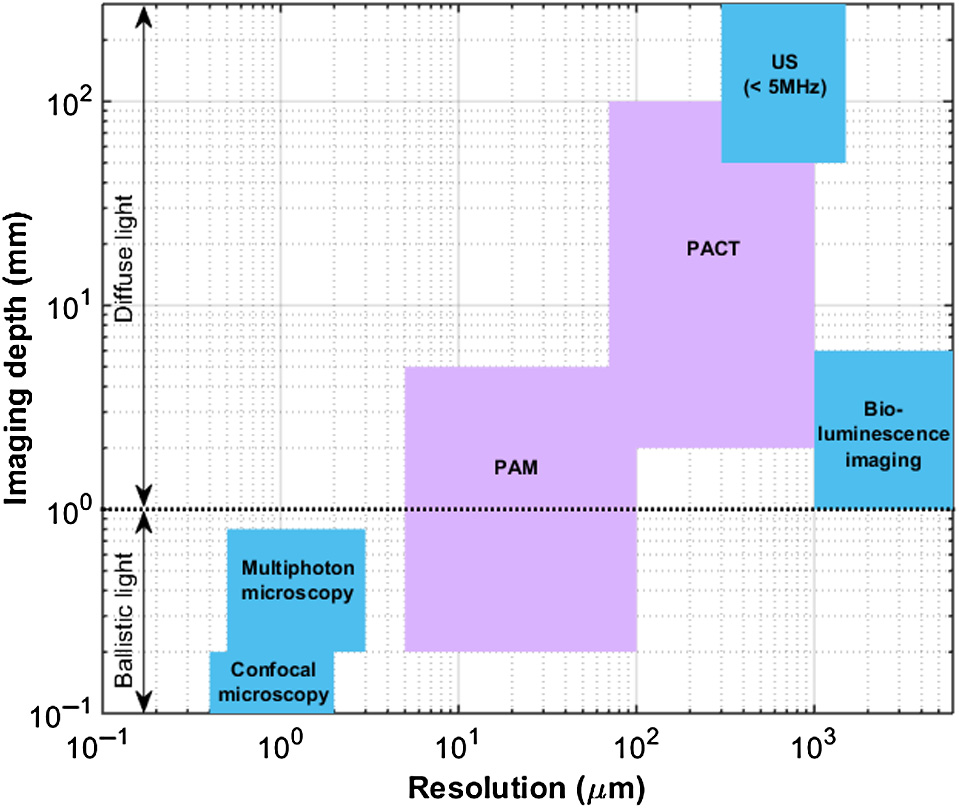
\includegraphics[width=0.5\columnwidth]{image/chap01/img_1_01.png}
	\caption{光声成像与其他成像技术在分辨率及深度上的对比\cite{brunker2017photoacoustic}}
	\label{img101}
\end{figure}

\subsubsection{光声成像技术对人体更安全}
现在广泛运用的成像方法都或多或少地对人体产生不好的影响。例如,X射线及CT具有较强的电离辐射,频繁使用会增加人体细胞的癌变风险等。但是由于光声成像产生的激光功率密度与超声场强度都远低于生物组织损伤阈值,所以光声成像是一种较安全、对人体无损的成像技术,能更好地服务于病人和医生。

\section{研究问题的发现及研究课题的提出}
\label{sec:related_work}
光声成像作为一项新兴的医学成像技术,在目前主要局限于研究领域,此时光声成像仪器的成本因素并不是主要考虑因素。但随着光声成像技术的日渐成熟,要想将光声成像技术广泛地应用于医疗卫生领域,其成本因素在实际推广的过程中往往不可忽视,有时甚至处于主导地位。虽然光声成像在实际的应用过程中具有其他现有成像方法所不具备的许多优势,但若在其推广的过程中无法控制应用成本,则必将受到层层阻碍。因此,如何降低光声成像的成本(包括设备成本、人力成本、耗材成本等),使得这项利民的医学技术能更快地使病人与医疗人员受益,是一项十分重要且有意义的工作。

因此,本文拟探究在低成本下得到高质量光声成像图像的方法,以降低光声成像技术在实际推广过程中的应用成本。

\subsection{光声成像重建算法问题的发现}
在前期的研究过程中发现,在现有的光声成像重建方法中,点状声波探测器的个数往往对重建效果起到关键性的影响。对点状声波探测器个数选用了50个、100个、200个、400个、800个的条件下(传感器阵列均采用围绕病灶排列且等距分布的中心圆),使用MatLab中的k-Wave对Skin Cancer MNIST数据集中选取的100张图片做光声成像的仿真以及重建,对得到的重建图像与原图像使用如MSE、SSIM、PSNR等指标进行评价,比较其在不同传感器个数下的成像质量。

我们挑选出其中一张皮肤癌图片,在不同传感器个数下的重建结果如图\ref{img102}。

\begin{figure}[h]
	\centering
	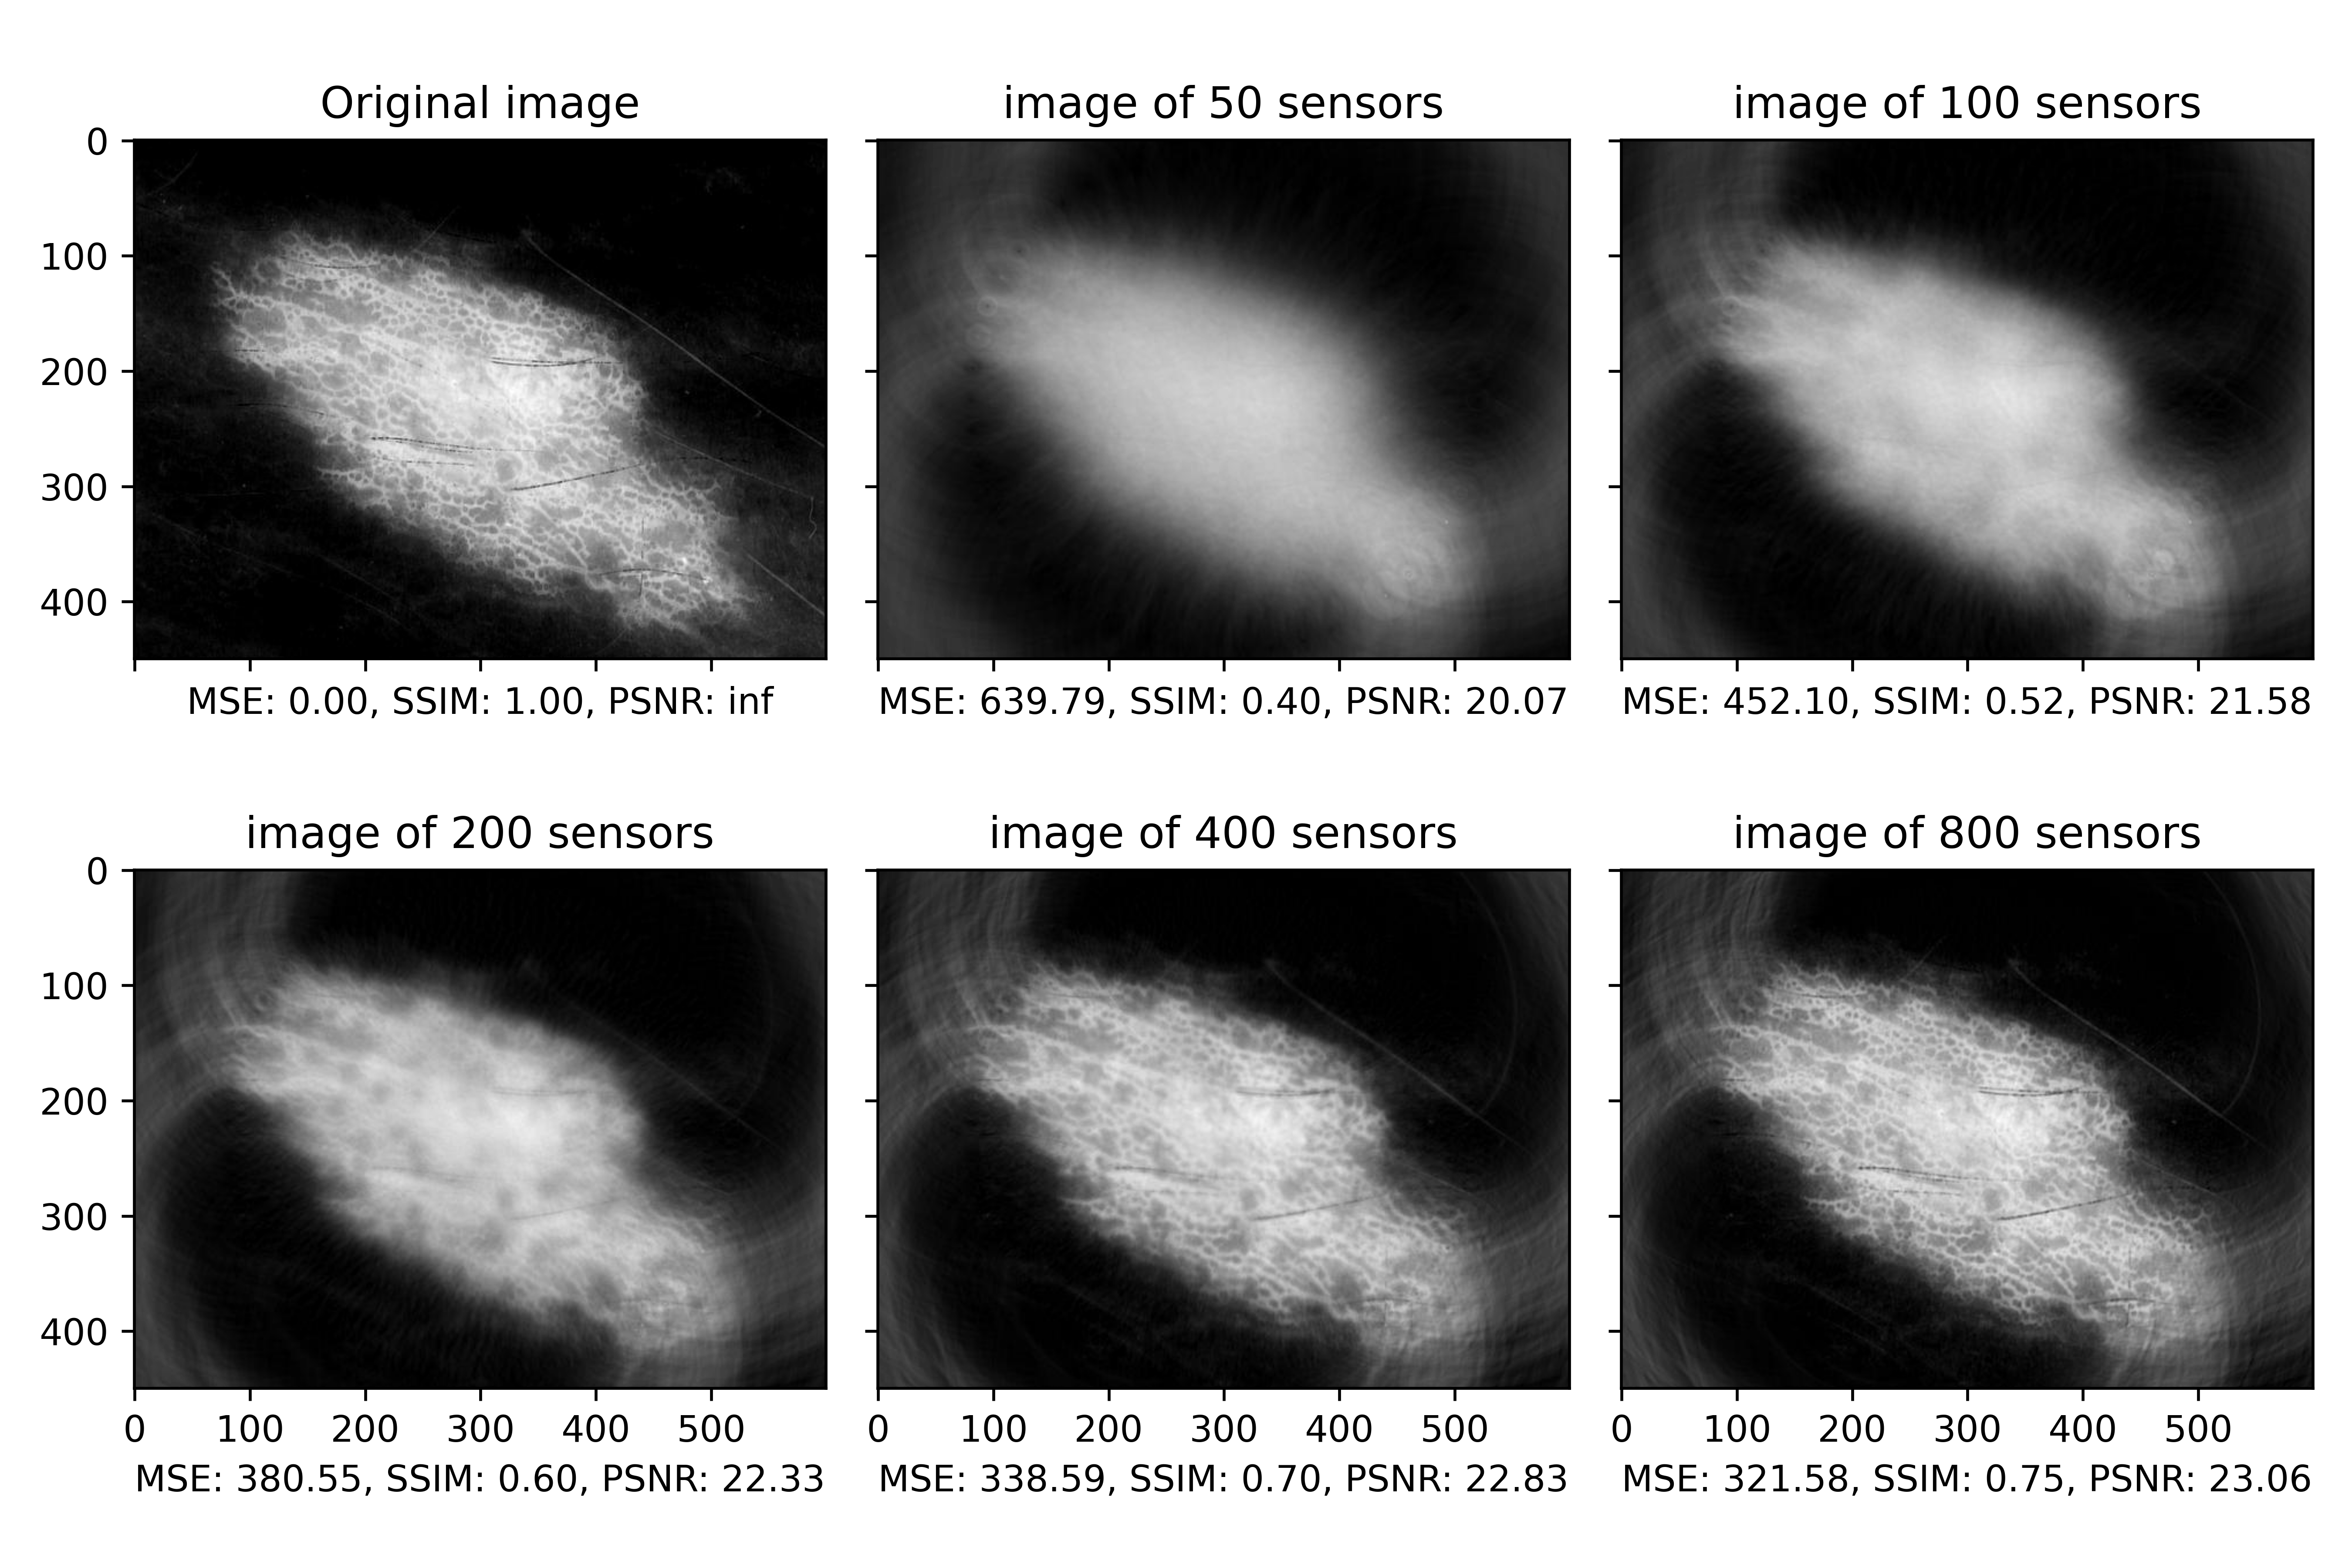
\includegraphics[width=0.75\columnwidth]{image/chap01/img_1_02.png}
	\caption{不同传感器数量下的重建图像}
	\label{img102}
\end{figure}

可以发现,随着传感器个数的减少,重建图片与原图片的MSE逐渐增加,SSIM、PSNR值逐渐降低,这说明该图片的成像质量不断降低。

为了排除单一案例造成的误差,我们计算出在不同传感器个数下,这100张重建图片与原图片的MSE、SSIM、PSNR的平均值。最终得到如图\ref{img103}的比较结果。

\begin{figure}[h]
	\centering
	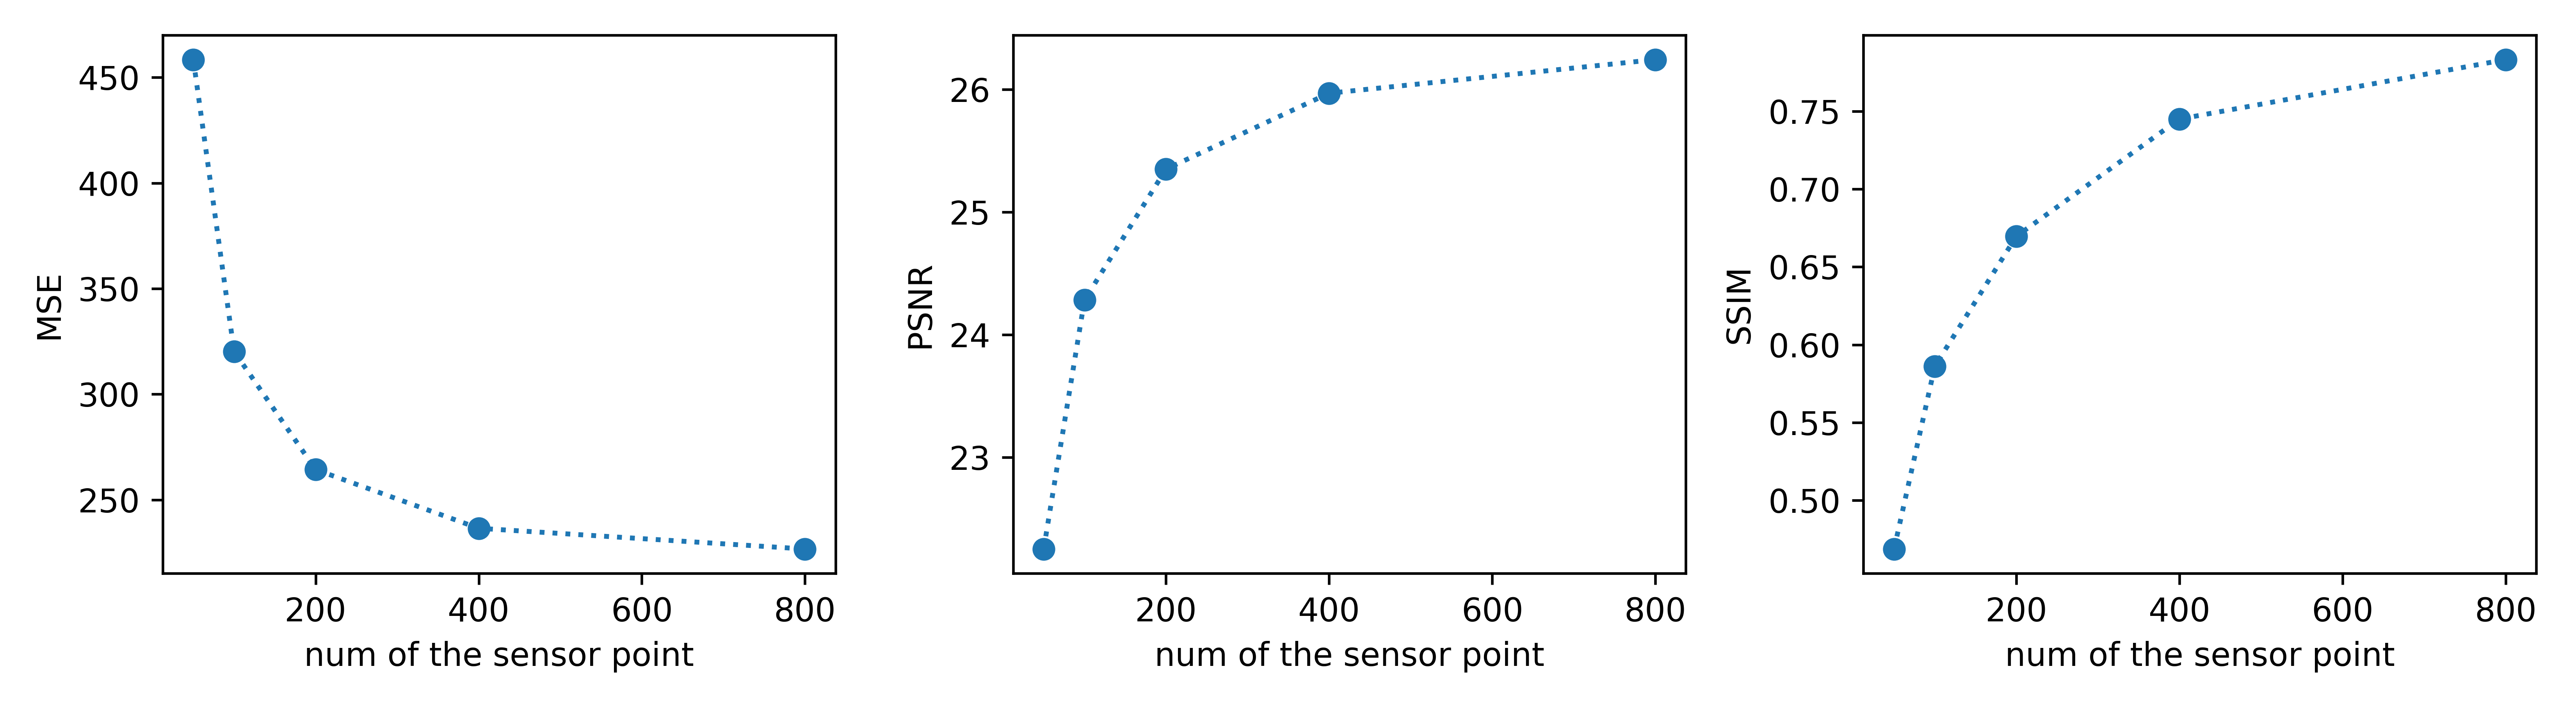
\includegraphics[width=0.9\columnwidth]{image/chap01/img_1_03.png}
	\caption{不同传感器数量下重建图像与原图像间的MSE、PSNR、SSIM}
	\label{img103}
\end{figure}

\hspace*{\fill} \

\hspace*{\fill} \

从图\ref{img103}的比较结果可知,当声波探测器的个数增加时,光声重建图像的MSE的均值呈现下降趋势,PSNR与SSIM的均值呈现上升趋势。这表明,传统光声成像重建算法的重建图像的精度和质量与仪器的声学传感器个数成正相关关系。并且可以得知,在声学传感器个数>=400个时,现有的算法重建的图像才具备较好的成像精度。

值得注意的是,上述结果是在没有为传感器数据添加噪声以及对图像进行任何降采样的情况下得出的。在实际情况中,由于传感器所接收到的数据信号往往会受到噪声的影响,重建效果往往更差。

\subsection{本项目研究课题的提出}
从上述观察可以看出,以现有的光声成像重建方法,重建的图像质量与光声成像仪器的声波探测器数量成正比。如果需要得到符合诊断标准的医学图像,就需要装备较多的声波探测器,从而进一步增加光声成像仪器的设备成本。

 如何利用较少传感器数量产生的较低精度光声重建图像,并将其优化为符合医学标准的光声重建图像就成为了本项目的出发点。对此,我们提出在图像处理领域,神经网络是一种成本较低的图像优化方案(神经网络的主要成本在于数据集的搭建及神经网络的训练)。并且由于神经网络的高延展性,在少量数据集上进行训练后的神经网络能有效应用到其他的数据集。因此,该方法能有效控制光声成像的应用成本。
 
 现今虽然已存在很多已训练的效果显著的图像优化网络。但由于医学图像的特殊性,若将这些神经网络直接运用于医学图像的优化,并使用优化后的医学图像进行疾病的诊断与治疗,不仅难以保证优化后的图像符合诊断标准,而且还有可能产生极大的医疗风险。因此,为光声成像单独搭建一组数据集并据此训练一套图像优化模型就显得十分必要了。
 
 综上所述,本项目的研究课题拟在搭建并训练一套神经网络模型,以实现将在低传感器数量下产生的低精度光声重建图像还原成高精度光声重建图像的目的。
 
 \section{基于深度学习的光声成像重建的研究现状}
 如今基于深度学习的光声成像图像重建主要有两大类研究方向:第一类是“可学习的非迭代重建”;第二类是“可学习的迭代重建”。
 \subsection{可学习的非迭代重建}
 对于光声成像的整个过程(如图\ref{img104}所示),可学习的非迭代重建主要有三种:
 
\begin{enumerate}
 	\item 增强测量信号:在重建的过程中,我们接受的信号可能存在畸变,如带宽的削减、噪声、通道数的跌落。于是我们可以通过深度学习的方法来将测量信号进行增强,如增强带宽、增强通道数。然后再对增强后的信号使用传统的重建方法重建。(图\ref{img104}橙色过程)
 	\item 学习逆过程:训练一个神经网络模型,来实现将接收到的信号传入,并直接输出重建图像的功能。(图\ref{img104}蓝色过程)
 	\item 增强重建图像:用神经网络对获取的重建图像进行增强,输出一个更高质量的图像。(图\ref{img104}绿色过程)
\end{enumerate}

\begin{figure}[h]
	\centering
	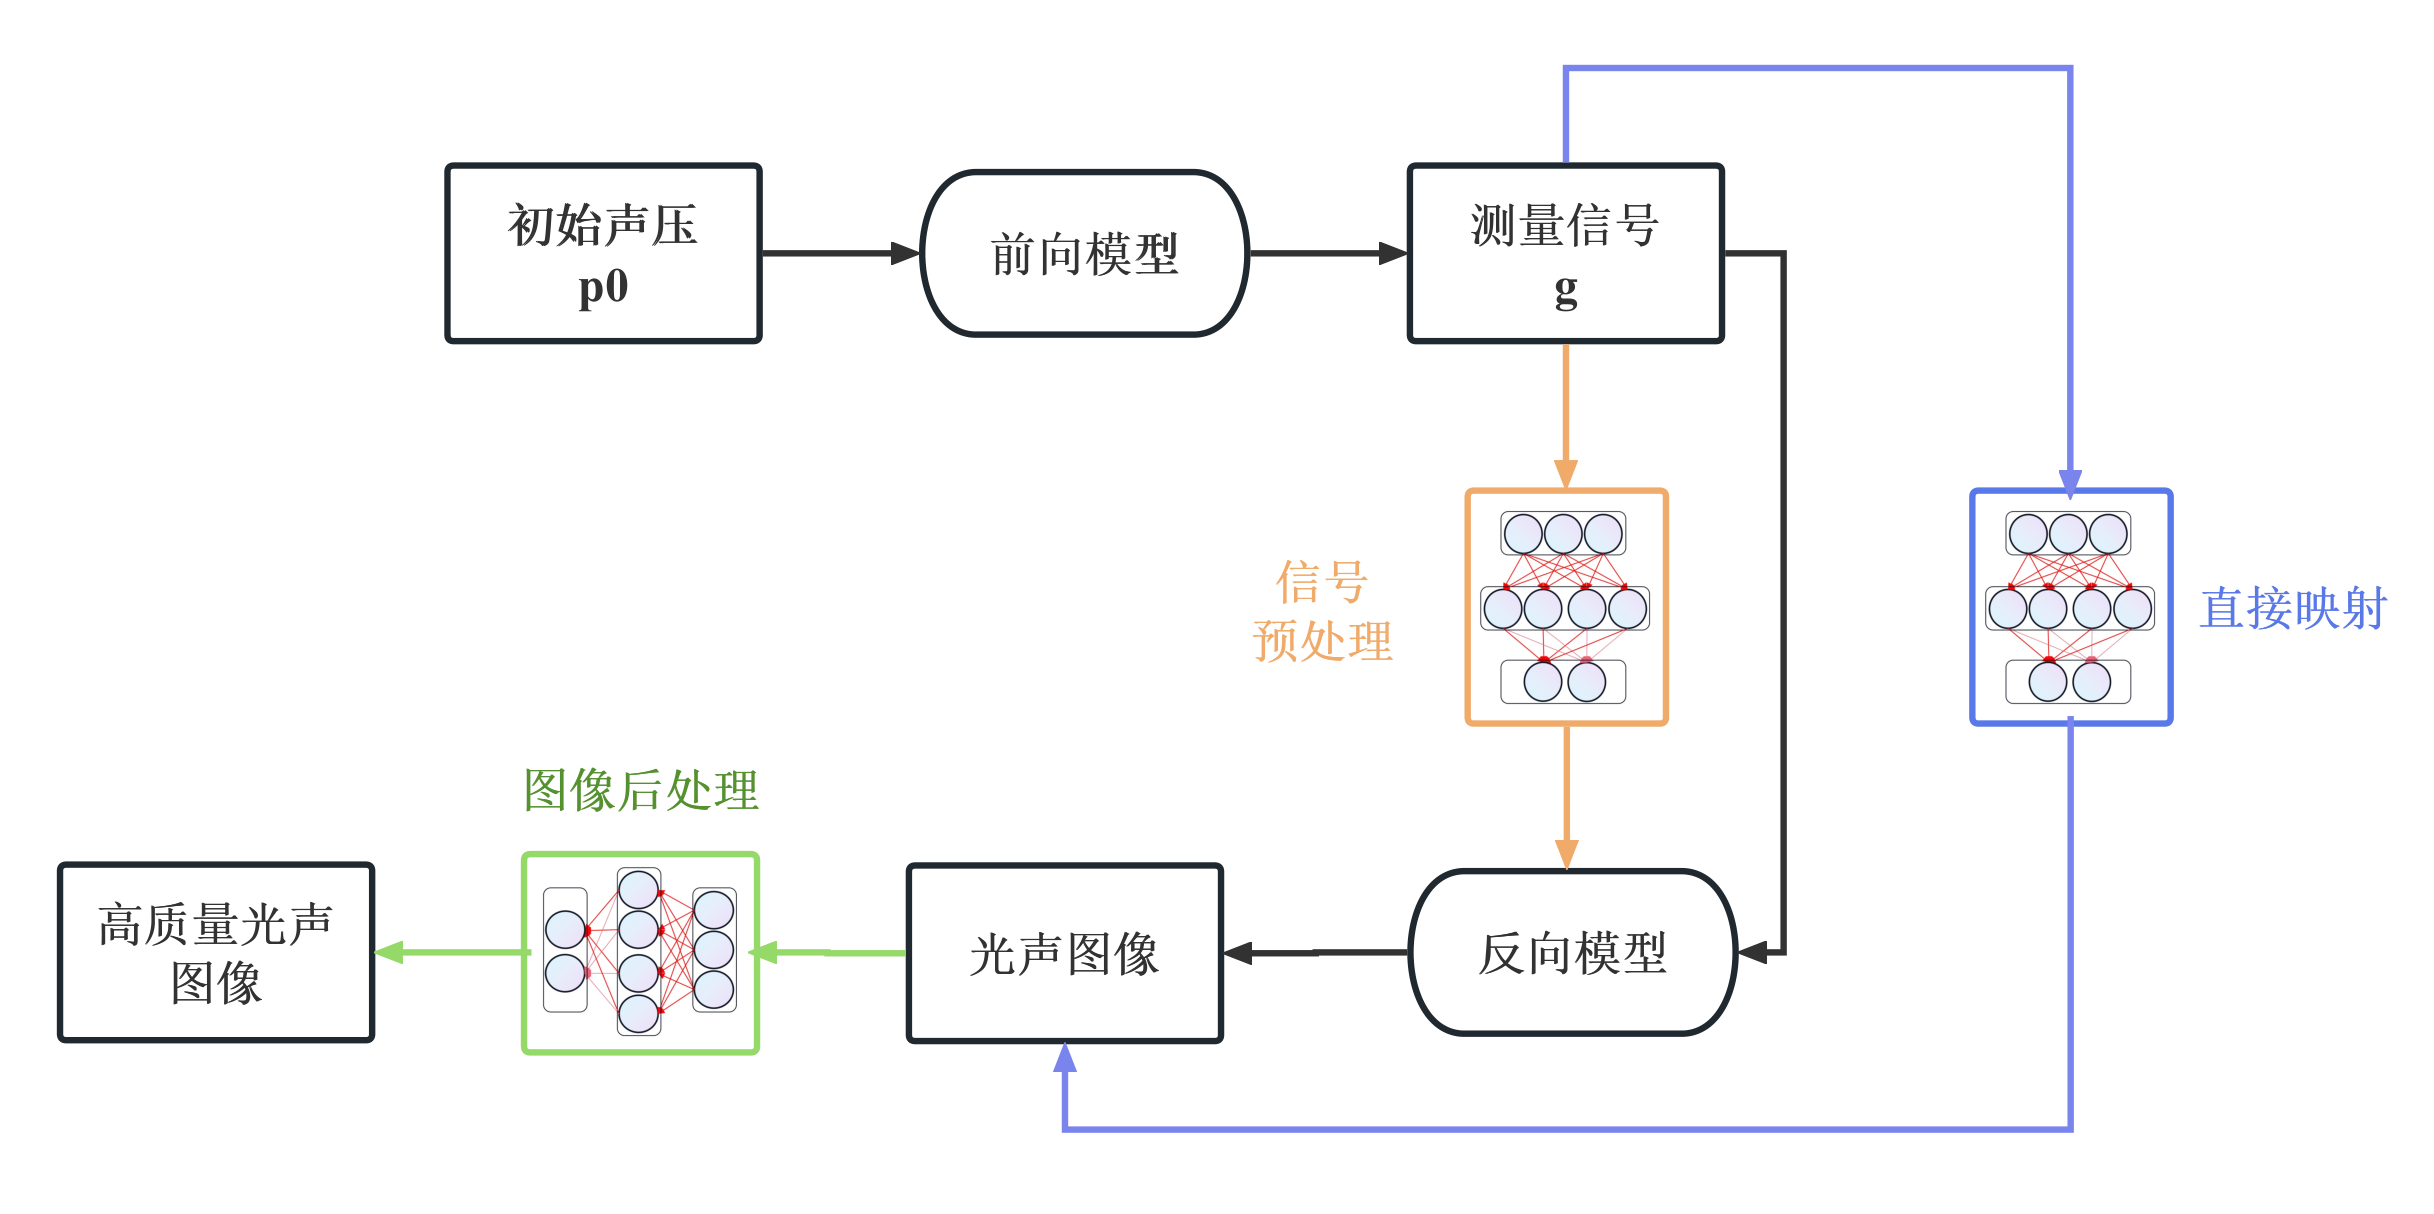
\includegraphics[width=0.9\columnwidth]{image/chap01/img_1_04.png}
	\caption{可学习的非迭代重建方案}
	\label{img104}
\end{figure}

\subsection{可学习的迭代重建}
可学习的迭代重建主要有两种:

\begin{enumerate}
	\item 利用深度学习学习重建过程中的优化方法(图\ref{img105}蓝色过程)
	\item 利用深度学习学习重建过程中的正则项(图\ref{img105}绿色过程)
\end{enumerate}

\begin{figure}[h]
	\centering
	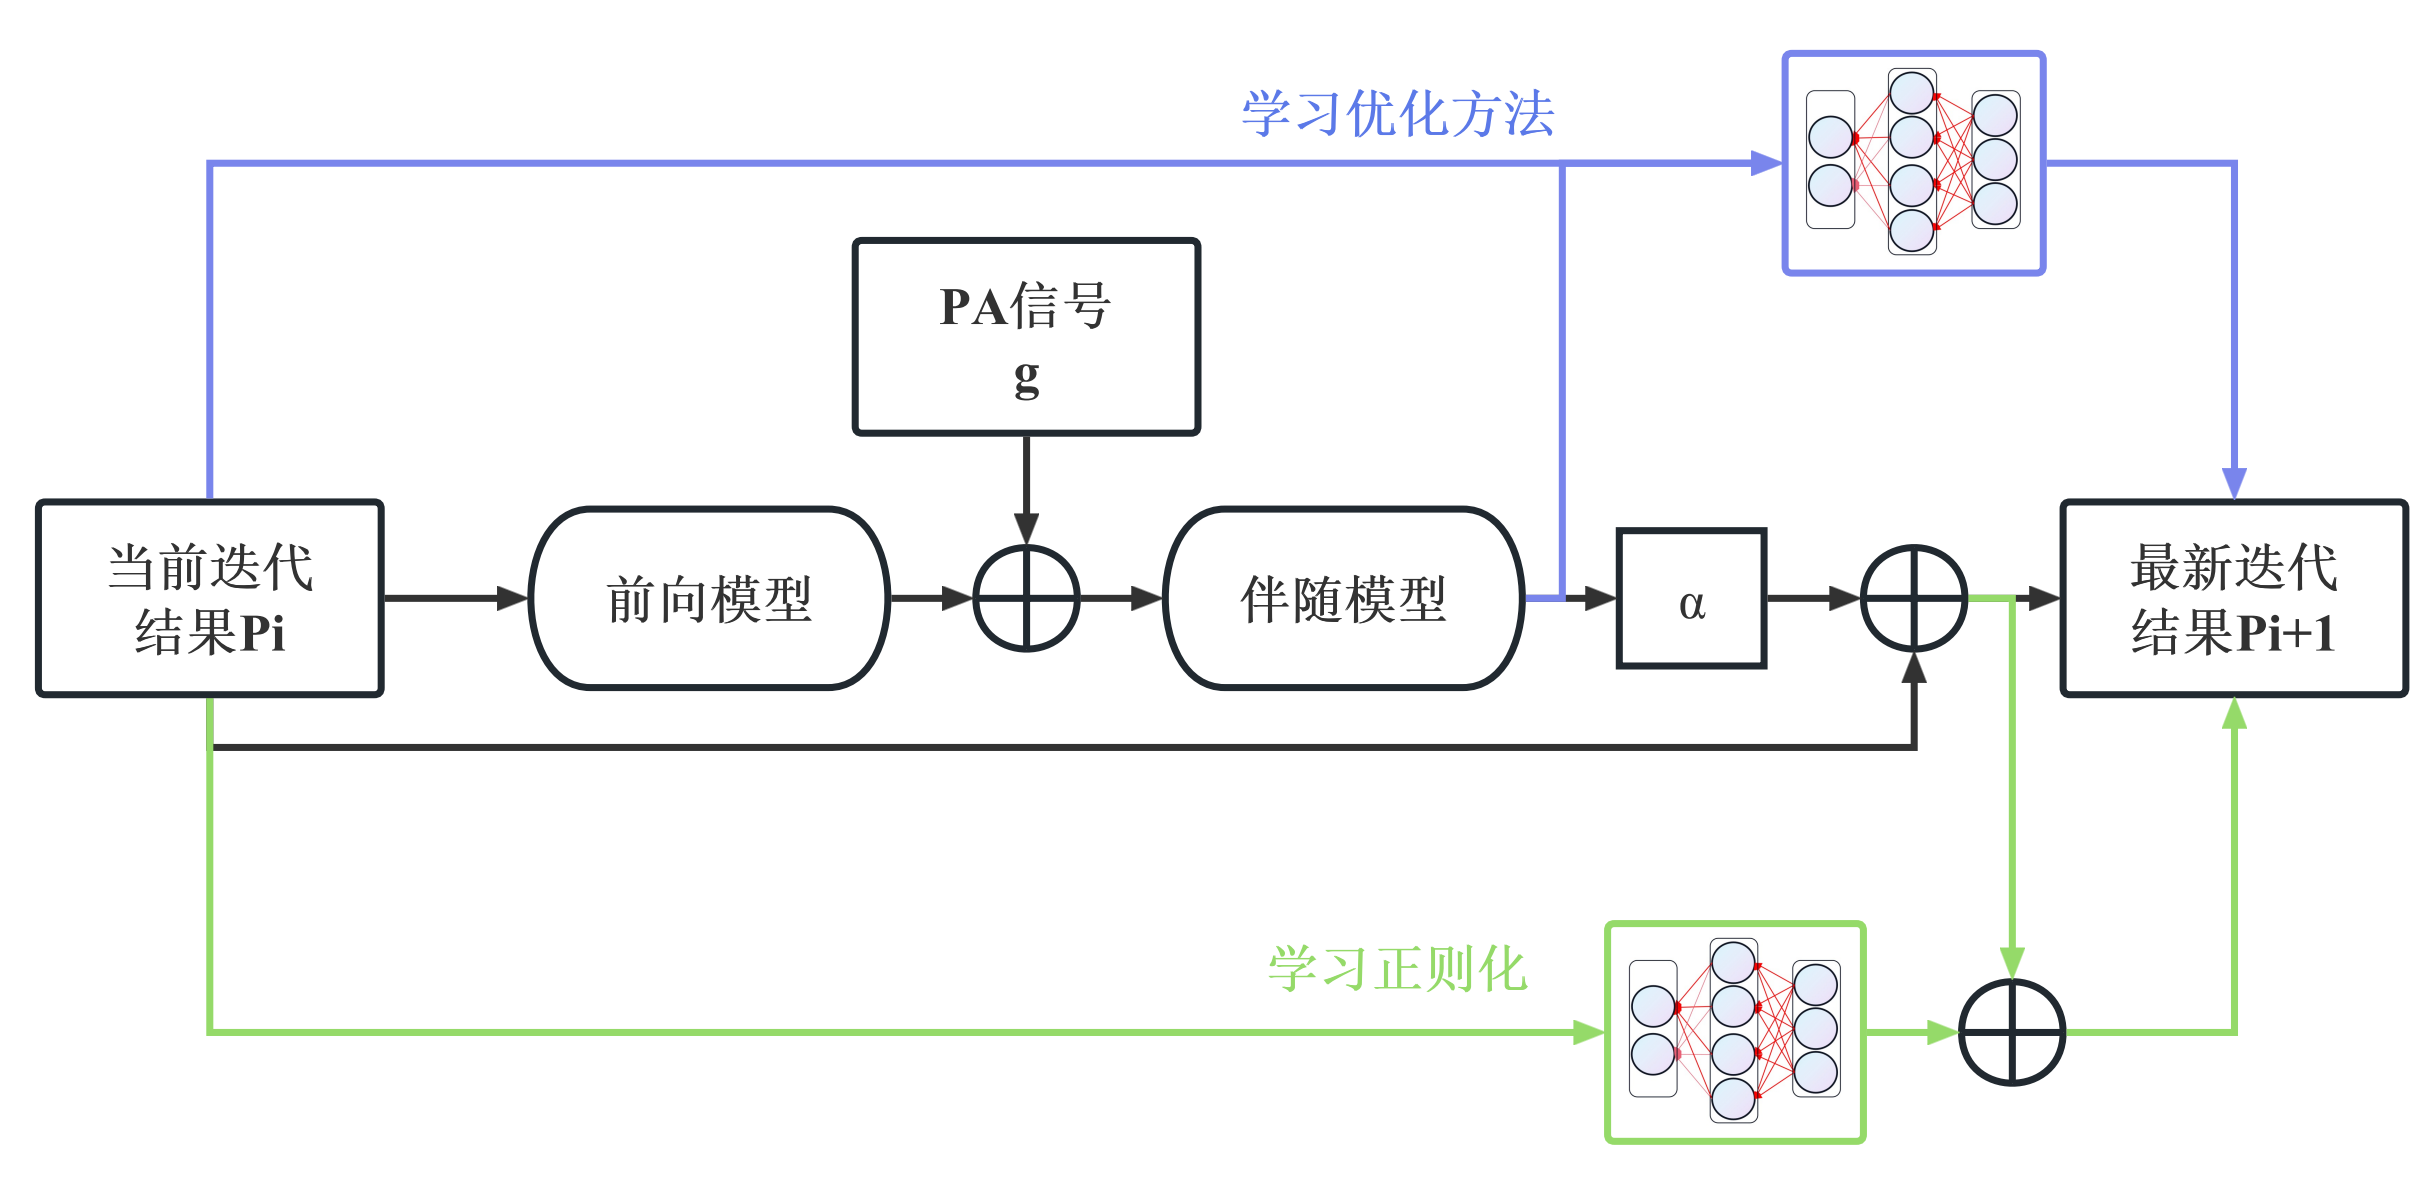
\includegraphics[width=0.9\columnwidth]{image/chap01/img_1_05.png}
	\caption{可学习的迭代重建方案}
	\label{img105}
\end{figure}

\subsection{本项目的研究现状}
在上述基于深度学习的光声成像重建方向中,本项目的研究课题是对非迭代重建方法中的后处理过程进行研究,以达到增强重建图像的研究目的。
   
关于利用深度学习进行光声成像的重建,现在也有不少的相关工作,比如用CNN来进行光声成像重建。而Transformer作为一个新兴的、热门的神经网络,在处理图像上超越了很多传统的神经网络模型。Transformer将自注意力机制引入CV领域,解决了以往神经网络诸如CNN无法很好地学习全局信息等缺点。Axial-Attention(轴向注意力)、ViT、Swin Transformer等不同的Transformer模型,都在计算机视觉领域取得了很大的成功,Swin Transformer更是其中的佼佼者。

因此,本项目拟将现今在CV领域效果卓越的Swin Transformer运用在光声成像重建后的图像优化,尝试并解决现今传统重建算法的各种问题。


\section{论文章节安排}

\label{sec:arrangement}

本文共分为六章,各章节内容安排如下:

第一章绪论。简单说明了本文章的选题背景与意义。

第二章阐述与光声成像有关的的理论基础,包括介绍光声成像的波动方程模型以及常见的几种光声成像重建算法等。

第三章主要介绍了Transformer模型的相关理论基础,包括Transformer模型中的注意力机制的理解与实现,及综述了现今将Transformer模型运用于CV领域的若干神经网络架构的实现原理。

第四章主要介绍该项目中利用MatLab及k-Wave搭建光声成像仿真与重建数据集的若干细节。

第五章主要介绍使用PyTorch实现Transformer模型并利用自建数据集进行训练的过程。

第六章的主要内容是对该Transformer模型的实验效果进行分析与评估。


